%%
%% Copyright 2007, 2008, 2009 Elsevier Ltd
%%
%% This file is part of the 'Elsarticle Bundle'.
%% ---------------------------------------------
%%
%% It may be distributed under the conditions of the LaTeX Project Public
%% License, either version 1.2 of this license or (at your option) any
%% later version.  The latest version of this license is in
%%    http://www.latex-project.org/lppl.txt
%% and version 1.2 or later is part of all distributions of LaTeX
%% version 1999/12/01 or later.
%%
%% The list of all files belonging to the 'Elsarticle Bundle' is
%% given in the file `manifest.txt'.
%%

%% Template article for Elsevier's document class `elsarticle'
%% with numbered style bibliographic references
%% SP 2008/03/01
%%
%%
%%
%% $Id: elsarticle-template-num.tex 4 2009-10-24 08:22:58Z rishi $
%%
%%
\documentclass[preprint,12pt,3p]{elsarticle}

%% Use the option review to obtain double line spacing
%% \documentclass[preprint,review,12pt]{elsarticle}

%% Use the options 1p,twocolumn; 3p; 3p,twocolumn; 5p; or 5p,twocolumn
%% for a journal layout:
%% \documentclass[final,1p,times]{elsarticle}
%% \documentclass[final,1p,times,twocolumn]{elsarticle}
%% \documentclass[final,3p,times]{elsarticle}
%% \documentclass[final,3p,times,twocolumn]{elsarticle}
%% \documentclass[final,5p,times]{elsarticle}
%% \documentclass[final,5p,times,twocolumn]{elsarticle}

%% if you use PostScript figures in your article
%% use the graphics package for simple commands
%% \usepackage{graphics}
%% or use the graphicx package for more complicated commands
%% \usepackage{graphicx}
%% or use the epsfig package if you prefer to use the old commands
%% \usepackage{epsfig}

%% The amssymb package provides various useful mathematical symbols
\usepackage{amssymb}
%% The amsthm package provides extended theorem environments
%% \usepackage{amsthm}

%% The lineno packages adds line numbers. Start line numbering with
%% \begin{linenumbers}, end it with \end{linenumbers}. Or switch it on
%% for the whole article with \linenumbers after \end{frontmatter}.
%% \usepackage{lineno}

%% natbib.sty is loaded by default. However, natbib options can be
%% provided with \biboptions{...} command. Following options are
%% valid:

%%   round  -  round parentheses are used (default)
%%   square -  square brackets are used   [option]
%%   curly  -  curly braces are used      {option}
%%   angle  -  angle brackets are used    <option>
%%   semicolon  -  multiple citations separated by semi-colon
%%   colon  - same as semicolon, an earlier confusion
%%   comma  -  separated by comma
%%   numbers-  selects numerical citations
%%   super  -  numerical citations as superscripts
%%   sort   -  sorts multiple citations according to order in ref. list
%%   sort&compress   -  like sort, but also compresses numerical citations
%%   compress - compresses without sorting
%%
%% \biboptions{comma,round}

% \biboptions{}

\usepackage{amsmath,bm}
\usepackage{hyperref}
\usepackage{subcaption}
\captionsetup{font={footnotesize,sf},labelfont={sf}}
\captionsetup[sub]{font={footnotesize,sf},labelfont={sf}}
\captionsetup[figure]{labelfont={bf},name={Fig.},labelsep=period}

\usepackage{cleveref}
\newcommand{\secref}[1]{section \ref{#1}}				% Referenz auf Kapitel
\newcommand{\figref}[1]{\hyperref[#1]{Fig. \ref*{#1}}}				% Referenz auf Abbildung
\newcommand{\tabref}[1]{table \ref{#1}}				% Referenz auf Tabelle
\newcommand{\subrefnew}[1]{(\subref*{#1})}

\hypersetup{
     colorlinks   = true,
     citecolor    = gray
}

\journal{Seminar Work CES, RWTH Aachen}

\begin{document}

\begin{frontmatter}

\title{Seminar Paper \\ \textbf{A phase-field model of dynamic fracture}}
\author[label1]{Karsten Paul (333092)}
\address[label1]{Computational Engineering Science (M.Sc.), RWTH Aachen \\ Supervisor: Christopher Zimmermann, M.Sc., AICES RWTH Aachen}
\ead{karsten.paul@rwth-aachen.de}

\begin{abstract}
Next to sharp interface models for the description and prediction of crack growth, diffuse interface models represent a powerful method so as to model cracks and their propagation. This work focuses on a phase-field description of dynamic fracture. Considering brittle fracture, the variational formulation of the problem is presented and the phase-field theory is introduced. A fourth-order model is exposed by extending the crack density functional of the second-order model. The resulting coupled systems of partial differential equations as well as the semidiscrete Galerkin forms are given. Since the fourth-order model requires a higher continuity of the phase-field's solution, a finite element analysis within an isogeometric analysis framework is outlined. A time integration scheme, based on the generalized-$\alpha$ method, is sketched for the description of dynamic fracture. The major differences between sharp and diffuse interface models are examined.
\end{abstract}

\begin{keyword}
%% keywords here, in the form: keyword \sep keyword
phase-field \sep fracture mechanics \sep variational formulation \sep brittle fracture \sep isogeometric analysis
%% MSC codes here, in the form: \MSC code \sep code
%% or \MSC[2008] code \sep code (2000 is the default)
\end{keyword}

\end{frontmatter}

%%
%% Start line numbering here if you want
%%
% \linenumbers

%% main text
\section{Introduction} \label{sec:intro}

So as to shorten development times, the prediction of fracture and failure in materials play a significant role for engineering designs. Mostly, experiments are not profitable due to high expense and enormous costs. So as to overcome these problems, computational models have been proposed in order to accurately model theses physical effects. 

% Sharp interface models
Finite Element Methods (FEM) are commonly used to numerically approximate crack behaviour in a given context. Here, a robust and efficient implementation is to the fore. A major question arising while modelling fracture processes within the FEM context is how to describe the splitting of the material. Obviously, it is not possible to simply let connected Finite Elements be separated from one point in time to the other. Thus, so called \textit{sharp interface models} have been proposed by enriching the displacement field with discontinuities or by inserting discontinuities by means of mesh handling. So as to give a short introduction to these approaches, subsequently, two of them are shortly outlined. Since these kind of strategies are not topic of this work, it is referred to \ref{appsec:sharp} where they are explained in a bit more detail.

The \textit{virtual crack closure technique} represents a crack by introducing one-dimensional discontinuities by a line of nodes. So as to let several Finite Elements separate from each other, there exist nodes with identical coordinates. In the case of undamaged material, multipoint constraints are imposed on these nodes so that they behave in the same manner. \cite{03_SotA_virtClos} 

In the \textit{cohesive segments method} the crack is represented by a set of overlapping cohesive segments. By means of these segments, displacement jumps are introduced as soon as the current stress state violates a given fracture criterion. However, this approach leads to several disadvantages: Quadrature rules have to be adapted, nodes need to have a variable number of degrees of freedom, there is a high accuracy error, the stress state at the tip of a segment is not well described and there is a problem is the specification of the geometry of the cohesive surfaces. \cite{02_SotA_cohes}\cite{01_SotA_cohes_dyn}

%\subsection{Fracture mechanics}
However, extending these formulations to three dimensions has proven to be difficult. Thus, today many approaches base on the variational formulation of brittle fracture. \citet{02_B_VarBrittle} propose that the solution of the fracture problem based on Griffith's theory is given by the minimizer of a global energy functional. In Griffith's theory a critical energy release rate determines crack nucleation and propagation. Accuracy and robustness of the variational formulation in two and three dimensions using the so called \textit{phase-field methods} which represents a diffuse interface model has been shown for instance by \citet{04_B_VarBrittleProve2} and \citet{03_B_VarBrittleProve1}. In there, a derivation of the phase-field based on continuum mechanics and thermodynamics is presented. Additionally, in \cite{04_B_VarBrittleProve2} the model distinguishing between tensile and compressive effects on crack growth has been established. Successful extensions to dynamic problems have been given by \citet{01_PF_dyn_brittle}, \citet{05_B_dynExtension1}, \citet{06_B_dynExtension2}, \citet{07_B_dynExtension3} and \citet{08_B_dynExtension4}. Actually, for example \citet{10_PH_Mode3} do not base their dynamic phase-field formulation on Griffith's theory of brittle fracture. However, this paper only deals with Griffith's theory as used for example by \citet{08_PF_Gammac2} since this theory is well understood and it has been proven to be useful in engineering applications \citep{01_PF_dyn_brittle}. The established phase-field models using the variational formulation of fracture have been widely numerically used and proved in different engineering contexts, for instance by \citet{11_B_EngProb1} and \citet{12_B_EngProb2} for hydraulic fracturing, by \citet{13_B_EngProb3} for piezoelectric ceramics, by \citet{14_B_EngProb4} for rubbery polymers and by \citet{15_B_EngProb5} for thermo-elastic solids. All these examples outline the relevance and the attractiveness of this formulation. In fact, for example \citet{03_PF_ductile} have shown that the phase-field method can also be used so as to model ductile fracture. Nevertheless, this work focuses on brittle fracture. A basic derivation of the governing equations considering ductile fracture is given in \ref{appsec:ductile}.

%\subsection{Phase-field theory}
In general, \textit{phase-field methods} are used so as to model interfaces between regions of different phases. Examples are the modelling of solidification behaviour, interfaces between fluids with different properties or, as discussed in this work, fracture. In the latter case, the interface describes the region between undamaged and totally broken material. Within the brittle fracture context, the phase-field theory can be seen as a regularization of the mentioned variational formulation. In there, the abrupt change between elastic behaviour and crack nucleation is smoothed as well as the boundary between undamaged and damaged material. Thus, no discontinuities are introduced into the body and the transition between two different phases is smoothed as it happens in a diffusive process. That is why the phase-field method belongs to the so called \textit{diffuse interface models}.

%\subsection{Isogeometric Analysis}
Isogeometric Analyis (IGA) is a powerful method in which functions used for the description of Computer Aided Design (CAD) geometries are adopted as a basis for analysis. Within the FEM context, no mesh generation is required and IGA allows for a high global regularity of the numerical solution. Especially, for $C^{2}$-continuity, standard Finite Elements quickly reach their beneficial properties. The IGA-framework has been established by \citet{09_B_IGA1}. The main concept lies in the usage of B-splines so as to model a geometry or, within the FEM context, in order to get a higher regularity using these functions as ansatz functions. The introduction of hierarchical B-Splines by \citet{18_IGA_HierBSplines} offered the possiblity of local refinement. This has then been expanded to locally refining NURBS (Non-Uniform Rational B-Splines). \citet{16_IGA_TSplines} have introduced so called T-Splines for the sake of a more efficient discretization of surfaces in contrast to hierarchical B-Splines. Local refinement strategies for these have been established as well as for NURBS, so called LR NURBS (Locally Refined NURBS) \cite{17_IGA_LRNURBS}.

% Fracture & IGA & phase-field
There exist many publications about fracture computations within an IGA framework. Just to mention two, \citet{19_B_FracIGA1} have developed an interface element based on IGA in the context of a sharp interface model of fracture and \citet{20_B_FracIGA2} have made use of an extended IGA (XIGA) framework for the sake of modelling dynamic fracture in multiphase piezoelectric/piezomagnetic composites. In \citet{11_PF_DissBorden} results of several papers concerning phase-field methods of dynamic fracture within an IGA framework are summarized. In there and in the corresponding papers \cite{03_PF_ductile}\cite{02_PF_HO_brittle}\cite{01_PF_dyn_brittle}, it has been observed that this complete framework works well for complex crack patterns and nucleation, even in three dimensions. By reason of a proposed higher order model, the used IGA framework by \citet{09_B_IGA1} has been proven to be very beneficial so as to achieve higher regularity in the numerical solution. In \cite{01_PF_dyn_brittle}, an adaptive refinement strategy using T-Splines has been proposed and numerically investigated.

% Outline of this work
In this work, firstly, the governing equations for obtaining stress equilibrium and for modelling the evolution of the phase-field are derived (\secref{sec:formul}). In there, brittle fracture is assumed and its variational formulation is outlined. Its minimizer is found by solving the Euler-Lagrange equation. At the end of \secref{sec:formul}, shortly, differences in modelling ductile fracture are pointed out. Since this works focuses on brittle fracture, a detailed derivation of the governing equationa for this type of fracture can be found in \ref{appsec:ductile}. \secref{sec:num_formul} focuses on the approximation of the solution of the governing equations including the derivation of the weak and semidiscrete Galerkin form. Shortly, a motivation for using an IGA framework so as to numerically solve these forms is given as well as a short introduction to IGA. Additionally, an appropriate time integration scheme for the given problem is given. This work finishes with \secref{sec:concl} by summarizing the phase-field model of dynamic fracture. Especially, phase-field methods of fracture are compared to sharp interface models of fracture so as to highlight the advantages of diffuse interface models for this type of problems.





\section{Formulation} \label{sec:formul}
The phase-field model as a diffuse interface model does not introduce discontinuities into the solid but the fracture surface is approximated by a scalar valued field. Thus, the boundary between damaged and not damaged areas is smoothed. In the following parts, a model for brittle and ductile fracture as well as a second- and fourth-order model are presented. At first, the notation and formulation considering brittle fracture is outlined. Afterwards, differences in the formulation considering ductile fracture are shown. For the rest of this paper, following notation is made (see \figref{fig:bodies}\subrefnew{fig:body_1}). The arbitraray body $\Omega\subset\mathbb{R}^{d}$ ($d\in\{1,2,3\}$) has external boundary $\partial\Omega$ and evolving internal discontinuity boundary (fracture surface) $\Gamma$. The displacement field at a given point $\mathbf{x}$ and time $t$ is given by $\mathbf{u}\left(\mathbf{x},t\right)\in\mathbb{R}^{d}$. Dirichlet boundary conditions $\mathbf{u}\left(\mathbf{x},t\right)=\mathbf{g}\left(\mathbf{x},t\right)$ on $\partial\Omega_{\mathbf{g}}$ and Neumann boundary conditions $\mathbf{t}\left(\mathbf{x},t\right)=\mathbf{h}\left(\mathbf{x},t\right)$ on $\partial\Omega_{\mathbf{h}}$ are imposed with $\partial\Omega_{\mathbf{g}}\cup\partial\Omega_{\mathbf{h}}=\partial\Omega$. $\mathbf{t}\left(\mathbf{x},t\right)$ describes a given traction vector force.
\begin{figure}[ht!]
    \centering
    \begin{subfigure}[t]{0.4\textwidth}
        \centering
        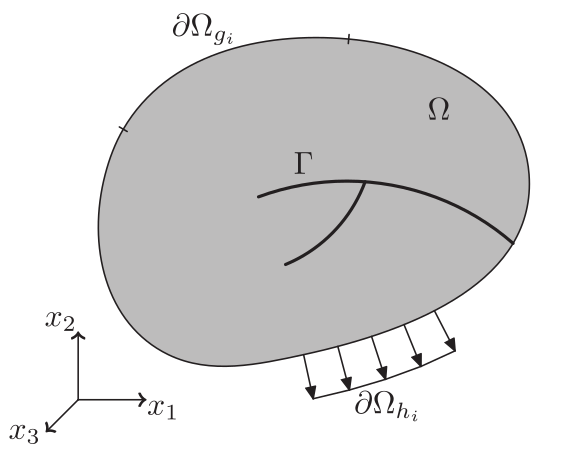
\includegraphics[scale=0.3]{data/Body_1}
        \caption{}\label{fig:body_1}
    \end{subfigure}
    %
    \begin{subfigure}[t]{0.5\textwidth}
        \centering
        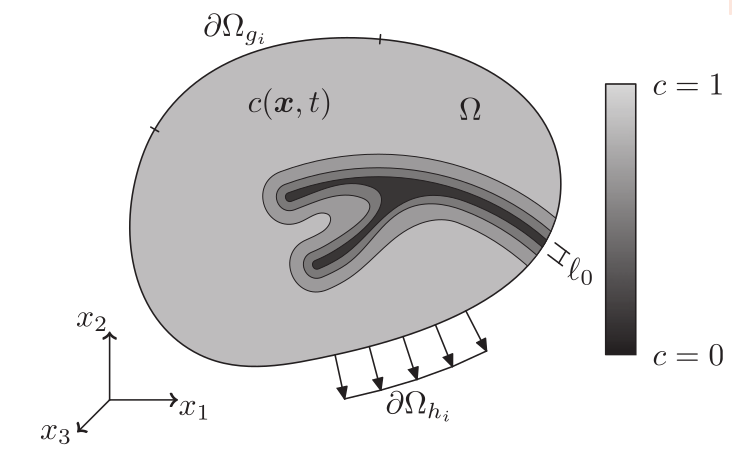
\includegraphics[scale=0.3]{data/Body_2}
        \caption{}\label{fig:body_2}
    \end{subfigure}
    \caption{\subrefnew{fig:body_1} Representation of a solid body $\Omega$ and internal discontinuitiy boundary $\Gamma$. \subrefnew{fig:body_2} Phase-field approximation of $\Gamma$. $c\left(\mathbf{x},t\right)$ describes the phase-field and $l_{0}$ is a parameter for controlling the failure zone's width. \cite{01_PF_dyn_brittle}} \label{fig:bodies}
\end{figure}


\subsection{Griffith's theory of brittle fracture} \label{sec:formul_Griffith}
Considering small derformations and deformation gradients, the small strain tensor $\bm{\varepsilon}\left(\mathbf{x},t\right)$ is given by
\begin{equation}
	\bm{\varepsilon} = \nabla^{s}\mathbf{u}
\end{equation}
where $\left(\cdot\right)^{s}$ refers to the symmetric part. Considering isotropic linear elasticity, the undamaged elastic energy densitiy can be expressed by
\begin{equation} \label{eq:psi_e}
	\Psi_ {e}\left(\bm{\varepsilon}\right) = \dfrac{1}{2}\lambda tr\left(\bm{\varepsilon}\right)^{2}+\mu\bm{\varepsilon}:\bm{\varepsilon}
\end{equation}
using the Lam\'{e} constants $\lambda$ and $\mu$ and $\left(\cdot\right):\left(\cdot\right)$ denoting the double contraction.

According to the energetic approaches to fracture, the critical fracture energy density $\mathcal{G}_{c}$ defines the energy being necessary to create a unit area of fracture surface. Since translation of cracks shall be forbidden and extension, branching and merging shall be allowed, there is an irreversibility condition stating $\Gamma\left(t\right)\subseteq\Gamma\left(t+\Delta t\right), \forall \Delta t>0$.

However, Griffith's fracture theory reaches its limits as soon as it is used to predict crack paths, nucleation of new cracks, complicated crack behaviours during kinking and branching. Thus, the problem is formulated in a variational sense which is shown in the following paragraphs. The phase-field approach can then be seen as a regularized version of this variational formulation. \citep{05_PF_ductile}

Newton's laws follow Hamilton's principle stating that the functional 
\begin{equation} \label{eq:fctal_Hamilton}
	J\left(q,\dot{q}\right)=\int\limits_{t_{0}}^{t_{1}}\mathcal{L}\left(q,\dot{q},t\right)\mathrm{d}t
\end{equation} reaches a stationary point. $\mathcal{L}\left(q,\dot{q},t\right)$ describes the so called Lagrangian and $q$ represents generalized coordinates. The motion of the mechanical system from $t_{0}$ to $t_{1}$ is then captured by this formulation \citep{01_B_LagrMech}. In our case, the Lagrangian reads $\mathcal{L}\left(\mathbf{u},\dot{\mathbf{u}},\Gamma\right)=\Psi_{kin}\left(\mathbf{u}\right)-\Psi_{pot}\left(\mathbf{u},\Gamma\right)$. Inserting the introduced cricical fracture energy densitiy $\mathcal{G}_{c}$, the kinetic energy of the body and \eqref{eq:psi_e} leads to
\begin{equation} \label{eq:lagr}
	\mathcal{L}\left(\mathbf{u},\dot{\mathbf{u}},\Gamma\right) = \int\limits_{\Omega}\left(\frac{1}{2}\rho\dot{\mathbf{u}}\dot{\mathbf{u}}-\Psi_{e}\left(\bm{\varepsilon}\right)\right)\mathrm{d}\Omega - \int\limits_{\Gamma}\mathcal{G}_{c}\mathrm{d}\Gamma.
\end{equation}
The Euler-Lagrange Equation (ELE) is a differential equation which solution satisfies equilibrium. Thus, this equation is also called the equation of motion \footnote{The term \textit{equation of motion} may be a bit misleading. It refers to the differential equation and not to its solution.}. A minimizer $q$ for \eqref{eq:lagr} satisfies the ELE
\begin{equation} \label{eq:ELE_O2}
	\dfrac{\partial\mathcal{L}}{\partial q}-\dfrac{\mathrm{d}}{\mathrm{d}t}\dfrac{\partial\mathcal{L}}{\partial\dot{q}}=0.
\end{equation}
For a given $\mathcal{L}=\mathcal{L}\left(q,\dot{q},\ddot{q}, t\right)$ this differential equation is changed to
\begin{equation} \label{eq:ELE:_O4}
	\dfrac{\partial\mathcal{L}}{\partial q}-\dfrac{\mathrm{d}}{\mathrm{d}t}\dfrac{\partial\mathcal{L}}{\partial\dot{q}}+\dfrac{\mathrm{d}^{2}}{\mathrm{d}t^{2}}\dfrac{\partial\mathcal{L}}{\partial\ddot{q}}=0
\end{equation}
\citep{01_B_LagrMech}. So as to circumvent problems of algorithmically tracking the propagating dicontinuity $\Gamma$, the phase-field approach will be presented in the next chapters which regularizes the just mentioned variational formulation.

\subsection{Phase-field approximation} \label{sec:ph_approx}
As can be seen in \figref{fig:bodies}\subrefnew{fig:body_2} the fracture surface $\Gamma$ is approximated by a scalar valued field $c\left(\mathbf{x},t\right)$. This field is called the phase-field. Values of $c=1$ represent regions away from the crack (undamaged material) whereas $c=0$ symbolizes the crack. Now, in \eqref{eq:lagr} the surface integral and thus, the need for tracking the crack can be eliminated. The approximation reads as follows:
\begin{equation} \label{eq:surf_int_approx}
	\int\limits_{\Gamma}\mathcal{G}_{c}\mathrm{d}\Gamma \approx \int\limits_{\Omega}\mathcal{G}_{c}\Gamma_{c,n}\mathrm{d}\Omega.
\end{equation}
Obviously, the surface integral can now be approximately calculated without knowing or tracking the fracture surface. \eqref{eq:surf_int_approx} represents the fracture surface energy. The quantity $\Gamma_{c,n}$ is called the crack density functional which depends on a parameter $l_{0}$, the phase-field $c\left(\mathbf{x},t\right)$ and its spatial derivatives up to order $\frac{n}{2}$ ($\frac{\partial c}{\partial \mathbf{x}},..,\frac{\partial^{\frac{n}{2}} c}{\partial \mathbf{x}^{\frac{n}{2}}}$). $l_{0}\in\mathbb{R}^{+}$ represents a parameter controlling the width of the approximation of the crack (see \figref{fig:bodies}\subrefnew{fig:body_2}). It could be seen as a numerical regularization parameter or as an material parameter. \citet{01_PF_dyn_brittle} showed that a critical stress level $\sigma_{c}$ depends on $l_{0}$. Thus, this parameter is here seen as a material property. For a more detailed discussion it refered to the investigations of \citet{07_PF_l0}.

The notation $\Gamma_{c,n}$ already presages that $n$ determines the order of the approximation. \citet{02_PF_HO_brittle} presented a so called \textit{second-} and \textit{fourth-order phase-field theory}. For $n=2$ the crack density functional introduced by \citet{08_PF_Gammac2} is used where as for $n=4$ a new functional has been established:
\begin{align}
	\begin{aligned}   \label{eq:crack_dens_fctals}
		\Gamma_{c,2} &= \dfrac{1}{4l_{0}}\left[\left(c-1\right)^{2}+4l_{0}^{2}|\nabla c|^{2}\right], \\
		\Gamma_{c,4} &= \dfrac{1}{4l_{0}}\left[\left(c-1\right)^{2}+2l_{0}^{2}|\nabla c|^{2}+l_{0}^{4}\left(\Delta c\right)^{2}\right].
	\end{aligned}
\end{align}
These formulations have been analytically analysed. So as to keep things short, it is referred to the work by \citet{02_PF_HO_brittle} for more detailed information. Only one important aspect is mentioned here: ${\eqref{eq:crack_dens_fctals}}_{1}$ is well-posed variationally for all $c\in H^{1}\left(\Omega\right)$ and solutions will generally not show greater regularity. Thus, ${\eqref{eq:crack_dens_fctals}}_{2}$ has been introduced so as to provide higher regularity in the solutions.

\subsection{Energy approximation} \label{sec:energy_approx}
In the failure zone there is a loss of material stiffness. So as to model this phenomena the elastic energy is split into contributions from tensile and compressive deformations\footnote{Originally, a parameter $k$ or $\eta<<1$ has been introduced by \citet{09_PF_k} into this equation so as to avoid ill-posedness. However, \citet{01_PF_dyn_brittle} found out that there is no necessity of setting $k>0$. Thus, the derivation of the governing evolution equations all include that $k=0$.}
\begin{equation} \label{eq:el_energy}
	\Psi_{e}\left(\bm{\varepsilon},c\right)=g\left(c\right) \Psi_{e}^{+}\left(\bm{\varepsilon}\right)+\Psi_{e}^{-}\left(\bm{\varepsilon}\right)
\end{equation}
with the so called degradation function $g\left(c\right)=c^{2}$. At a later point in this work there will be more information on this function. This splitting is achieved with the help of spectral decomposition of the strain:
\begin{align} \label{eq:spectr_decomp}
	\begin{aligned}
		\bm{\varepsilon} = \mathbf{P}\bm{\Lambda}\mathbf{P}^{T} \quad \Rightarrow \quad \bm{\varepsilon}^{+} = \mathbf{P}\bm{\Lambda}^{+}\mathbf{P}^{T},  \bm{\varepsilon}^{-} = \mathbf{P}\bm{\Lambda}^{-}\mathbf{P}^{T}, \\
		\bm{\Lambda}^{+}=diag\left(\left<\lambda_{1}\right>,\left<\lambda_{2}\right>,\left<\lambda_{3}\right>\right), \quad \left<x\right>=\begin{cases}x, &x>0 \\ 0, & x\leq0\end{cases}.
	\end{aligned}
\end{align}
$\bm{\Lambda}^{-}$ is analogously                                                                                                                                                                                                                                                                                                                                                                                                                                                                                                          defined. $\lambda_{i}\in\sigma\left(\bm{\varepsilon}\right),i\in\{1,2,3\}$ denote the eigenvalues of the strain tensor. Plugging \eqref{eq:spectr_decomp} into \eqref{eq:psi_e} leads to the energy contributions from tensile and compressive deformations:
\begin{align} \label{eq:psi_e+-}
	\begin{aligned}
		\Psi_{e}^{+}\left(\bm{\varepsilon}\right) &= \dfrac{1}{2}\lambda\left<tr\left(\bm{\varepsilon}\right)\right>^{2}+\mu tr\left[\left(\bm{\varepsilon}^{+}\right)^{2}\right], \\
		\Psi_{e}^{-}\left(\bm{\varepsilon}\right) &= \dfrac{1}{2}\lambda\left(tr\left(\bm{\varepsilon}\right)-\left<tr\left(\bm{\varepsilon}\right)\right>\right)^{2}+\mu tr\left[\left(\bm{\varepsilon}-\bm{\varepsilon}^{+}\right)^{2}\right].
	\end{aligned}
\end{align}
The assumption here is that the sign of the principal straings determine tensile and compressive contributions. Putting \eqref{eq:el_energy} and \eqref{eq:surf_int_approx} together leads to the Helmholtz free energy given by
\begin{equation} \label{eq:Helmholtz}
	\Psi_{n}=c^{2}\Psi_{e}^{+}+\Psi_{e}^{-}+\mathcal{G}_{c}\Gamma_{c,n}.
\end{equation}

\subsection{Strong form} \label{sec:strong_form}
The governing equations will be one for enforcing stress equilibrium and the other will govern the phase-field evolution.

Assuming given body forces $\mathbf{b}$ and traction vector forces $\mathbf{t}=\bm{\sigma}\mathbf{n}$ with outward-pointing normal vector on $\partial\Omega$, stress equilibrium is enforced by
\begin{equation} \label{eq:stress_equil}
	 \left\{\begin{alignedat}{2}
\nabla\cdot\bm{\sigma}+\mathbf{b} &= \rho\ddot{\mathbf{u}} && \quad\text{on } \Omega\times\left(0,T\right) \\
		\mathbf{u} &= \mathbf{g} && \quad\text{on } \partial\Omega_{\mathbf{g}}\times\left(0,T\right) \\
		\bm{\sigma}\mathbf{n} &= \mathbf{h} && \quad\text{on } \partial\Omega_{\mathbf{h}}\times\left(0,T\right) \\
		\mathbf{u} &= \mathbf{u}_{0} && \quad\text{on } \Omega\times0 \\
		\dot{\mathbf{u}} &= \mathbf{v}_{0} && \quad\text{on } \Omega\times0.
  \end{alignedat}\right.
\end{equation}
$\eqref{eq:stress_equil}_{1}$ represents the local form of the linear momentum balance with $\bm{\sigma}=c^{2}\frac{\partial\Psi_{e}^{+}}{\partial\bm{\varepsilon}}+\frac{\partial\Psi_{e}^{-}}{\partial\bm{\varepsilon}}$.

As described in \secref{sec:formul_Griffith}, the Euler-Lagrange Equation can be used to find a minimizer of \eqref{eq:fctal_Hamilton}. Plugging \eqref{eq:crack_dens_fctals} and \eqref{eq:el_energy} into \eqref{eq:lagr} as well as using \eqref{eq:surf_int_approx} makes the use of the ELE possible. For this case, $q\hat{=}c$ and $\frac{\mathrm{d}}{\mathrm{d}t}\hat{=}\frac{\mathrm{d}}{\mathrm{d}\mathbf{x}}$. All this together lead to the governing equations for the evolution of the phase-field, namely $\eqref{eq:c2_equil}_{1}$ for the second- and $\eqref{eq:c4_equil}_{1}$ for the fourth-order phase-field theory. As can be seen in these equations, $\Psi_{e}^{+}$ has been replaced by strain histroy field $\mathcal{H}$ enforcing the irreversibility condition $\Gamma\left(t\right)\subseteq\Gamma\left(t+\Delta t\right), \forall \Delta t>0$ in the strong form. This field satisfies the Kuhn-Tucker conditions for loading and unloading \cite{01_PF_dyn_brittle}:
\begin{equation} \label{eq:KuhnTucker}
	\Psi_{e}^{+}-\mathcal{H}\leq0, \quad \dot{\mathcal{H}}\geq0, \quad \dot{\mathcal{H}}\left(\Psi_{e}^{+}-\mathcal{H}\right)=0.
\end{equation}
It can also be used to model pre-existing cracks or geometrical features \cite{01_PF_dyn_brittle}.

 \hl{\text{Boundary-Conditions!}}
\begin{equation} \label{eq:c2_equil}
		 \left\{\begin{alignedat}{2}
\left(\frac{4l_{0}\mathcal{H}}{\mathcal{G}_{c}}+1\right)c - 4l_{0}^{2}\Delta c &= 1 && \quad\text{on } \Omega\times\left(0,T\right) \\
\hl{\nabla c\cdot\mathbf{n}} &= 0 && \quad \text{on } \partial\Omega\times\left(0,T\right) \\
\mathcal{H} &= \mathcal{H}_{0} && \quad \text{on } \Omega\times0  
\end{alignedat}\right.
\end{equation}
\begin{equation} \label{eq:c4_equil}
		 \left\{\begin{alignedat}{2}
\left(\frac{4l_{0}\mathcal{H}}{\mathcal{G}_{c}}+1\right)c - 2l_{0}^{2}\Delta c + l_{0}^{4}\Delta\left(\Delta c\right) &= 1 && \quad\text{on } \Omega\times\left(0,T\right) \\
\hl{\Delta c} &= 0 && \quad \text{on } \partial\Omega\times\left(0,T\right) \\
\hl{\nabla\left(l_{0}^{4}\Delta c-2l_{0}^{2}c\right)\cdot\mathbf{n}} &= 0 && \quad \text{on } \partial\Omega\times\left(0,T\right) \\
\mathcal{H} &= \mathcal{H}_{0} && \quad \text{on } \Omega\times0  
\end{alignedat}\right.
\end{equation}
The numerical approximation of the solution of \eqref{eq:c2_equil} and \eqref{eq:c4_equil} are outlined in \secref{sec:num_formul}. The last topic of the next section is the difference in modelling ductile fracture in contrast to brittle fracture which has been considered up to this point.

\subsection{Ductile fracture} \label{sec:ductile_frac}
So as to motivate this section, at first the differences between the modelling of brittle and ductile fracture are examined. Up to this point of this paper, linear elasticity has been assumed. In this context, brittle fracture has been formulated in a variational way. By introducing the phase-field approximation, a regularized formulation of the variational one has been established. The corresponding stress-strain-curves and the procedure are illustrated in \figref{fig:elastic}.
\begin{table}[!ht]
	\begin{center}
	\begin{tabular}{|c||c|c|c|}
		\cline{2-4}
			\multicolumn{1}{c||}{}& Linear elasticity & \multicolumn{2}{c|}{Brittle fracture} \\
 		\hline\hline
			\rotatebox[origin=c]{90}{ Process} & \raisebox{-.5\height}{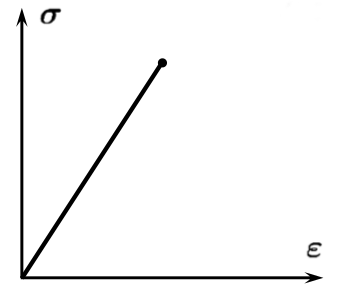
\includegraphics[scale=0.3]{data/elastic_1}} & \raisebox{-.5\height}{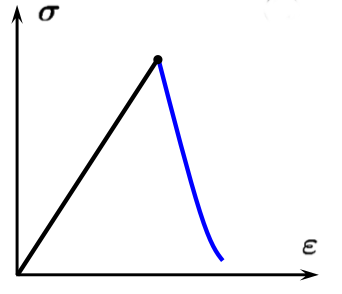
\includegraphics[scale=0.3]{data/elastic_2}} & \raisebox{-.5\height}{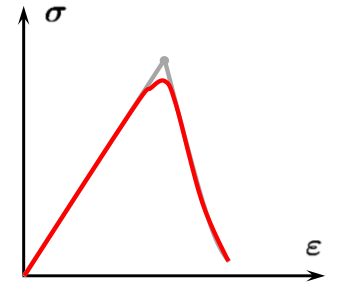
\includegraphics[scale=0.3]{data/elastic_3}} \\
		\hline
			\rotatebox[origin=c]{90}{\small{ Formulation }} & $E\left(\mathbf{u}\right)$ & \begin{tabular}[c]{@{}c@{}}Variational formulation\\of brittle fracture\\$E\left(\mathbf{u},\Gamma\right)$\end{tabular}  & \begin{tabular}[c]{@{}c@{}}Phase-field formulation\\($\hat{=}$regularized version)\\$E\left(\mathbf{u},c\right)$\end{tabular} \\
		\hline
	\end{tabular}
	\end{center}
\captionof{figure}{Brittle fracture: Process from linear elasticity over the variational formulation towards the phase-field approximation. \cite{06_PF_ductile}} \label{fig:elastic}
\end{table}
The variational formulation has been well established. Thus, the regularized version using the phase-field approximation could be found. As the dashed lines in \figref{fig:plastic} reveal, there is no variational formulation of ductile fracture found yet. Thus, the foundation of the regularized version is not as easy as for brittle fracture.

\begin{table}
	\begin{center}
	\begin{tabular}{|c||c|c|c|}
		\cline{2-4}
			\multicolumn{1}{c||}{}& Plasticity & \multicolumn{2}{c|}{Ductile fracture} \\
 		\hline\hline
			\rotatebox[origin=c]{90}{ Process} & \raisebox{-.5\height}{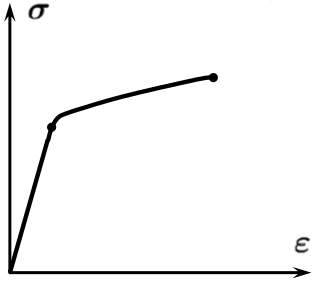
\includegraphics[scale=0.3]{data/plastic_1}} & \raisebox{-.5\height}{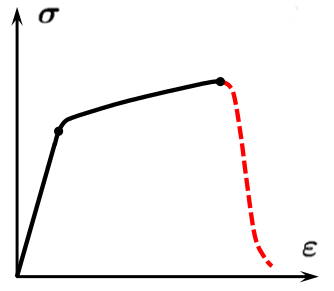
\includegraphics[scale=0.3]{data/plastic_2}} & \raisebox{-.5\height}{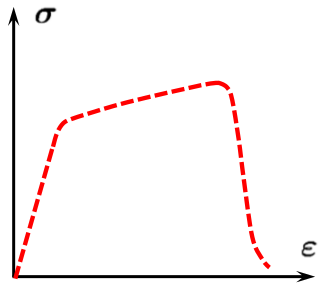
\includegraphics[scale=0.3]{data/plastic_3}} \\
		\hline
			\rotatebox[origin=c]{90}{\small{ Formulation }} & $E\left(\bm{\varepsilon}^{e},\bm{\varepsilon}^{p},\alpha\right)$ & \begin{tabular}[c]{@{}c@{}}Variational formulation\\of ductile fracture\\$E\left(\bm{\varepsilon}^{e},\bm{\varepsilon}^{p},\alpha,\Gamma\right)$\end{tabular}  & \begin{tabular}[c]{@{}c@{}}Phase-field formulation\\($\hat{=}$regularized version)\\$E\left(\bm{\varepsilon}^{e},\bm{\varepsilon}^{p},\alpha,c\right)$\end{tabular} \\
		\hline
	\end{tabular}
	\end{center}
\captionof{figure}{Ductile fracture: Process from plasticity towards the phase-field approximation. The variational formulation has not been established yet. \cite{06_PF_ductile}} \label{fig:plastic}
\end{table}

\citet{06_PF_ductile} proposes a method similar to the one presented here for brittle fracture. The major change lies in the Helmholtz free energy (see \eqref{eq:Helmholtz}) which is replaced by
\begin{equation} \label{eq:Helmholtz_ductile1}
	\Psi_{n} = g\left(c,p\right)\Psi_{e}^{+}\left(\bm{\varepsilon}\right)+\Psi_{e}^{-}\left(\bm{\varepsilon}\right)+\Psi_{p}\left(\alpha\right)+\mathcal{G}_{c}\Gamma_{c,n}
\end{equation}
with the new degradation function $g\left(c,p\right)c^{2p}+\eta$ and $p=\frac{\epsilon_{eq}^{p}}{\epsilon_{eq,crit}^{p}}$, $\epsilon_{eq}^{p}\left(t\right)=\sqrt{\frac{2}{3}}\int\limits_{0}^{t}\sqrt{\dot{\bm{\varepsilon}}:\dot{\bm{\varepsilon}}}\mathrm{d}t$. The plastic energy density function considering linear isotropic hardening reads $\Psi_{p}\left(\alpha\right)=\sigma_{y}\alpha+\frac{1}{2}h\alpha^{2}$ with yield stress $\sigma_{y}$, hardening variable $\alpha$ and hardening modulus $h>0$. The idea in this new degradation function is that $c$ depends on $p$ so that the fracture process can be seen as the accumulation of ductile damage. $\Psi_{p}$ will take the dominating role over $\Psi_{e}^{+}$ and thus, a plasticity-driven fracture initiation is achieved. However, here a more abstract derivation of the governing equations will be presented which is based on the work of \citet{03_PF_ductile}.

In \secref{sec:formul_Griffith} small deformations and deformation gradients have been assumed. Since this does not hold true for ductile fracture, another approach for the derivation of the strong form is chosen. As \citet{03_PF_ductile} have outlined, previous approaches on ductile fracture suffer in the fact that yield surface and hardening modulus are not effected by the phase-field's evolution. Thus, at some point plastic strains saturate and deformation is again dominated by revoverable elastic strains. The notation mentioned at the beginning of this section stays the same. The deformation gradient, which cannot be considered small anymore, now reads
\begin{equation} \label{eq:deform_grad}
	\mathbf{F}=\dfrac{\partial\varphi\left(\mathbf{X},t\right)}{\partial\mathbf{X}}
\end{equation}
with deformation map $\varphi:\left(\Omega_{0}\times\mathbb{R}\right)\rightarrow\mathbb{R}^{d}$, body $\Omega_{0}$ in the reference configuration  and $\mathbf{x}=\varphi\left(\mathbf{X},t\right)$. \eqref{eq:deform_grad} is now decomposed into elastic and plastic deformations gradiend
\begin{equation} \label{eq:deform_grad_decomp}
	\mathbf{F}=\mathbf{F}^{e}\mathbf{F}^{p}
\end{equation}
Compared to \eqref{eq:Helmholtz}, the new stored energy functional proposed by \citet{03_PF_ductile} reads
\begin{equation} \label{eq:fctal_ductile}
	\tilde{\Psi}\left(\mathbf{F},c,c_{,\mathbf{X}},\mathbf{F}^{p},\alpha\right) = \int\limits_{\Omega_{0}}\left[g\left(c\right)\Psi^{+}\left(\mathbf{F},\mathbf{F}^{p}\right)+\Psi^{-}\left(\mathbf{F},\mathbf{F}^{p}\right)+g_{p}\left(c\right)\Psi_{p}\left(\alpha\right)+\Gamma_{c,n}\right]\mathrm{d}\Omega_{0}
\end{equation}
with $\left(\cdot\right)_{\mathbf{X}}$ denoting the derivative with respect to $\mathbf{X}$\footnote{Note that for ductile fracture in this work, $\nabla\left(\cdot\right)$ is replaced by $\left(\cdot\right)_{,\mathbf{X}}$ or $\left(\cdot\right)_{,\mathbf{x}}$, respectively in order to distinguish between derivatives with respect to the reference or current configuration. For brittle fracture, everything has been derived within the current configuration.}. As in the work by \citet{06_PF_ductile}, an effective plastic work contributation $\Psi_{p}$ depending on the internal hardening variable $\alpha$ has been added. The plastic degradation function $g_{p}\left(c\right)$ provides, analogously to $g\left(c\right)$ a mechanism invoving crack growth driven by development of plastic strains. For example, $g\left(c\right)$ leads to the neglection of plastic softening. In \citep{03_PF_ductile} it has been examined that $g\left(c\right)=c^{2}$ is not leading to a linear stress-strain-curve up to the point of critical stress. To overcome this problem, \citet{03_PF_ductile} propose following parameterized cubic degradation function:
\begin{equation} \label{eq:cubic_degr_fct}
	g\left(c\right)=m\left(c^{3}-c^{2}\right)+3c^{2}-2c^{3}
\end{equation}
with $m>0$ determining the slope of $g$ at $c=1$. It can be shown that for strains smaller the critical strain for the quadratic degradation function the cubic degradation function leads to $\sigma=E\varepsilon$ as $m\rightarrow0$. Thus, $m=10{-4}$ has been chosen in their numerical examples. The two major accomplishments using the cubic degradation function are at first, there is a nearly linear stress-strain behaviour up to the point of critical stress. Thus, linear elasticity is modelled more accurately. Secondly, it shows up that the critical stress is higher than for the quadratic degradation function (for $l_{0}$ fixed). Thus, a larger length scale parameter can be used so as to achieve the critical stress since $\sigma_{crit}^{cubic}\sim l_{0}^{-\frac{1}{2}}$. Thus, coarser meshes can be used in order to reduce computational effort.

The approach for the derivation of the governing equations is based on balance laws. To keep things short, not every single step of their derivation but more likely their results are presented here. Microfoce balance laws are assumed to model the phase-field's evolution within a large deformation setting. The balance of linear momentum and angular momentum in the reference configuration lead to (also see \eqref{eq:stress_equil})
\begin{equation} \label{eq:lin_mom_ang_mom}
	\begin{aligned}
		Div\left(\mathbf{P}\right)+\mathbf{B}&=\rho_{0}\ddot{\mathbf{U}}, \\
		\bm{\sigma} &= \bm{\sigma}^{T}
	\end{aligned}
\end{equation}
with $1^{st}$ Piola-Kirchhoff stress tensor $\mathbf{P}$, density $\rho_{0}$ in the reference configuration and $Div\left(\cdot\right)$ denoting the divergence in the reference configuration. Analogously, assuming an internal microforce $\pi\left(\mathbf{x},t\right)\in\mathbb{R}$, an external microforce $l\left(\mathbf{x}.t\right)\in\mathbb{R}$ acting on the body and an external microforce $\lambda\left(\mathbf{x},t\right)=\bm{\xi}\cdot\mathbf{N}$ acting on the surface (with microforce traction vector $\bm{\xi}\left(\mathbf{x},t\right)\in\mathbb{R}^{d}$), the microfoce balance leads to
\begin{equation} \label{eq:microforce_balance}
	Div\left(\bm{\xi}\right)+\pi+l=0.
\end{equation}
The energy balance with $e$ describing the internal energy per unit volume reads
\begin{equation} \label{eq:energy_balance}
	\int\limits_{\Omega_{0}}\dot{e}_{0}\mathrm{d}\Omega_{0}=\int\limits_{\Omega_{0}}\mathbf{P}:\dot{\mathbf{U}}\mathrm{d}\Omega_{0}+\int\limits_{\partial\Omega_{0}}\lambda\dot{c}\text{ }\mathrm{d}\partial\Omega_{0}+\int\limits_{\Omega_{0}}l\dot{c}\text{ }\mathrm{d}\Omega_{0},
\end{equation}
where $\dot{c}$ is the work conjugate of the microforces. The second law of thermodynamics leads to
\begin{equation}
	\Theta\dot{s}\geq0
\end{equation}
with entropy per unit volume $s$ and absolute temperature $\Theta$. Note that heat fluxes and heat sources are not considered here (isothermal and adiabatic process). Using the dissipation inequality $e_{0}=\Psi+\Theta  s$ (see Legendre transormation) this can be rewritten as
\begin{equation} \label{eq:entropy_balance}
	\dot{\Psi}\leq\dot{e}_{0}
\end{equation}
with Helmholtz free energy $\Psi$. Using \eqref{eq:energy_balance} and \eqref{eq:entropy_balance}, applying the divergence theorem, integrating by party and using \eqref{eq:microforce_balance}, a thermodynamically consistent model is achieved as long as $\Psi$ fulfills \hl{wieso U. -> F.}
\begin{equation} \label{eq:thermodyn_cons}
		\int\limits_{\Omega_{0}}\dot{\Psi}\mathrm{d}\Omega_{0} \leq \int\limits_{\Omega_{0}}\left(\mathbf{P}:\dot{\mathbf{F}}+\bm{\xi}\cdot\dot{c}_{,\mathbf{X}}-\pi\dot{c}\right)\mathrm{d}\Omega_{0} = \int\limits_{\Omega_{0}}\left(\dfrac{1}{2}\mathbf{S}:\dot{\mathbf{C}}+\bm{\xi}\cdot\dot{c}_{,\mathbf{X}}\pi\dot{c}\right)\mathrm{d}\Omega_{0}.
\end{equation}
$\mathbf{S}$ denotes the $2^{nd}$ Piola-Kirchhoff stress tensor and $\mathbf{C}=\mathbf{F}^{T}\mathbf{F}$ the right Cauchy-Green tensor.

Assuming that $\Psi=\Psi\left(\mathbf{C},\mathbf{C}^{p},\mathbf{Q},c,c_{,\mathbf{X}},\dot{c}\right)$ with plastic right Cauchy-Green tensor $\mathbf{C}^{p}={\mathbf{F}^{p}}^{T}\mathbf{F}^{p}$ and set of internal plastic variables $\mathbf{Q}$, applying the chain rule in \eqref{eq:thermodyn_cons} leads to
\begin{equation} \label{eq:thermodyn_cons2}
	\begin{aligned}
	\int\limits_{\Omega_{0}}&\left(\dfrac{\partial\Psi}{\partial\mathbf{C}}:\dot{\mathbf{C}}+\dfrac{\partial\Psi}{\partial\mathbf{C}^{p}}:\dot{\mathbf{C}}^{p}+\dfrac{\partial\Psi}{\partial\mathbf{Q}}\cdot\dot{\mathbf{Q}}+\dfrac{\partial\Psi}{\partial c}\dot{c}+\dfrac{\partial\Psi}{\partial c_{,\mathbf{X}}}\cdot\dot{c}_{,\mathbf{X}}+\dfrac{\partial\Psi}{\partial\dot{c}}\ddot{c}\right)\mathrm{d}\Omega_{0} \\
	&\leq \int\limits_{\Omega_{0}}\left(\dfrac{1}{2}\mathbf{S}:\dot{\mathbf{C}}+\bm{\xi}\cdot\dot{c}_{,\mathbf{X}}-\pi\dot{c}\right)\mathrm{d}\Omega_{0}.
	\end{aligned}
\end{equation}
by applying the chain rule and integrating over the reference domain $\Omega_{0}$.

The plastic dissipation $\mathbb{D}^{p}=-\dfrac{\partial\Psi}{\partial\mathbf{C}^{p}}:\dot{\mathbf{C}}^{p}-\dfrac{\partial\Psi}{\partial\mathbf{Q}}\cdot\dot{\mathbf{Q}}$ can be set to zero for purely elastic deformations. Comparing the terms on the left hand and right hand side of \eqref{eq:thermodyn_cons2}, the following relations can be derived:
\begin{equation} \label{eq:relations_cons2}
	\begin{aligned}
		\dfrac{\partial\Psi}{\partial\dot{c}} &= 0, \\
		\dfrac{\partial\Psi}{\partial c_{,\mathbf{X}}} &= \bm{\xi}, \\
		2\dfrac{\partial\Psi}{\partial\mathbf{C}} &= \mathbf{S}, \\
		\left(\pi+\dfrac{\partial\Psi}{\partial c}\right)\dot{c} &\leq 0, \\
		\mathbb{D}^{p} &\geq 0.
	\end{aligned}
\end{equation}
$\eqref{eq:relations_cons2}_{4}$ can be rewritten as
\begin{equation} \label{eq:relation_cons_beta}
	\pi = -\dfrac{\partial\Psi}{\partial c}-\beta\dot{c}
\end{equation}
with function $\beta=\beta\left(\mathbf{C},\mathbf{C}^{p},c,c_{,\mathbf{X}}\right)\geq0$\footnote{$\beta$ can be seen as a dissipation constant.}. Inserting \eqref{eq:relations_cons2} and \eqref{eq:relation_cons_beta} into the balance laws $\eqref{eq:lin_mom_ang_mom}_{1}$ and \eqref{eq:microforce_balance}, leads to following equations (using $\mathbf{P}=\mathbf{F}\mathbf{S}$):
\begin{equation} \label{eq:balance_laws}
	\begin{aligned}
		Div\left(2\mathbf{F}\dfrac{\partial\Psi}{\partial\mathbf{C}}\right)+\mathbf{B} &= \rho_{0}\ddot{\mathbf{U}}, \\
		Div\left(\dfrac{\partial\Psi}{\partial c_{,\mathbf{X}}}\right)+l-\dfrac{\partial\Psi}{\partial c} &= \beta\dot{c}.
	\end{aligned}
\end{equation}
Considering \eqref{eq:fctal_ductile}, the Helmholtz free energy for ductile fracture reads
\begin{equation} \label{eq:Helmholtz_ductile2}
	\Psi_{n}\left(\mathbf{C},\mathbf{C}^{p},\mathbf{Q},c,c_{,\mathbf{X}}\right) = g\left(c\right)\Psi^{+}\left(\mathbf{C},\mathbf{C}^{p}\right)+\Psi^{-}\left(\mathbf{C},\mathbf{C}^{p}\right)+g_{p}\left(c\right)\Psi_{p}\left(\mathbf{Q}\right)+\Gamma_{c,n}.
\end{equation}
For the fourth-order phase-field theory $\Psi$ also depends on the second-order spatial derivatives of $c$. Using this, the partial derivatives required in \eqref{eq:balance_laws} can be computed. Furthermore, setting $l=0$ and $\beta=0$ leads to the governing equations. The stress equilibrium is given by
\begin{equation} \label{eq:stress_equil_ductile}
	 \left\{\begin{alignedat}{2}
		Div\left(2\mathbf{F}\left(g\left(c\right)\dfrac{\partial\Psi^{+}}{\partial\mathbf{C}}+\dfrac{\partial\Psi^{-}}{\partial\mathbf{C}}\right)\right)+\mathbf{B} &= \rho_{0}\ddot{\mathbf{U}} && \quad\text{on } \Omega_{0}\times\left(0,T\right) \\
		\mathbf{U} &= \mathbf{G} && \quad\text{on } \partial\Omega_{0,\mathbf{G}}\times\left(0,T\right) \\
		\mathbf{T} &= \mathbf{H} && \quad\text{on } \partial\Omega_{0,\mathbf{H}}\times\left(0,T\right) \\
		\mathbf{U} &= \mathbf{U}_{0} && \quad\text{on } \Omega_{0}\times0 \\
		\dot{\mathbf{U}} &= \mathbf{V}_{0} && \quad\text{on } \Omega_{0}\times0.
  \end{alignedat}\right.
\end{equation}
with Piola-Kirchhoff traction vector $\mathbf{T}=\mathbf{P}\cdot\mathbf{N}$. Considering the second-order phase-field theory and inserting the two partial derivatives $\frac{\partial\Psi}{\partial c_{,\mathbf{X}}}$ and $\frac{\partial\Psi}{\partial c}$ required in \eqref{eq:balance_laws} with the help of \eqref{eq:Helmholtz_ductile2} leads to following equation:
\begin{equation} \label{eq:c2_ph_evolution_tmp}
\dfrac{2l_{0}}{\mathcal{G}_{c}^{0}}\left(g'\left(c\right)\Psi^{+}+g_{p}'\left(c\right)\Psi_{p}\right) + c - 4l_{0}^{2}\Delta c = 1 \quad\text{on } \Omega\times\left(0,T\right).
\end{equation}
However, the irreversibility conditions outlined in \eqref{eq:KuhnTucker} have not been considered yet. Now, the history field is given by
\begin{equation} \label{eq:history_field_ductile}
	\mathcal{H}\left(\mathbf{C},\mathbf{C}^{p}\right) = \max\limits_{\bar{t}\leq t} \Psi^{+}\left(\mathbf{C}\left(\bar{t}\right),\mathbf{C}^{p}\left(\bar{t}\right)\right).
\end{equation}
Having $\left<\cdot\right>$ defined as in \eqref{eq:spectr_decomp}, the term $\Psi_{p}$ in \eqref{eq:c2_ph_evolution_tmp} is replaced by $\left<\Psi_{p}-\Psi_{0}\right>$. Actually, $\Psi_{p}$ is already assumed to be monotonically increasing so that no additional constraints are necessary in order to enforce irreversibility crack growth caused by plastic deformation. However, \citet{03_PF_ductile} introduce the plastic work threshold $\Psi_{0}$ so as to have more control over the contribution of plastic deformation to crack growth. Thus, if $\Psi_{p}<\Psi_{0}$, there will be no contribution of plastic deformation to crack growth. This point can now be controlled easily. Furthermore, \citet{03_PF_ductile} introduce parameters $\beta_{e}\in\left[0,1\right]$ and $\beta_{p}\left[0,1\right]$ which can be used in order to weight the contributions from elastic strain energy and plastic work to crack growth. These modifications, \eqref{eq:c2_ph_evolution_tmp} and \eqref{eq:history_field_ductile} lead to the governing equations for the evolution of the phase-field considering ductile fracture and the second-order phase-field theory:
\begin{equation} \label{eq:c2_equil_ductile}
	\left\{\begin{alignedat}{2}
		\dfrac{2l_{0}}{\mathcal{G}_{c}^{0}}\left(\beta_{e}g'\left(c\right)+\beta_{p}g_{p}'\left(c\right)\left<\Psi_{p}-\Psi_{0}\right>\right) + c - 4l_{0}^{2}\Delta c\ &= 1 && \quad\text{on } \Omega_{0}\times\left(0,T\right) \\
		\hl{c_{,\mathbf{X}}\cdot\mathbf{N}} &= 0 && \quad \text{on } \partial\Omega_{0}\times\left(0,T\right) \\
		\mathcal{H} &= \mathcal{H}_{0} && \quad \text{on } \Omega_{0}\times0,
	\end{alignedat}\right.
\end{equation}
There are several constitutive models so as to determine the energy densitiy functions $\Psi^{+}$, $\Psi^{-}$ and $\Psi_{p}$. These have been well outlined by \citet{03_PF_ductile} and within this work, it is only referred to this work. \hl{initial condition right?! or u0 v0 sufficient? -> dissertation Borden}

Since $\eqref{eq:crack_dens_fctals}_{2}$ includes second order spatial derivatives for the fourth-order phase-field theory, the relations \eqref{eq:relations_cons2} have to be adapted. For that, the Helmholtz free energy is assumed to take the form $\Psi=\Psi\left(\mathbf{C},\mathbf{C}^{p},\mathbf{Q},c,c_{,\mathbf{X}},c_{,ii},\dot{c}\right)$.
\begin{equation} \label{eq:thermodyn_cons4}
	\begin{aligned}
	\int\limits_{\Omega_{0}}&\left(\dfrac{\partial\Psi}{\partial\mathbf{C}}:\dot{\mathbf{C}}+\dfrac{\partial\Psi}{\partial\mathbf{C}^{p}}:\dot{\mathbf{C}}^{p}+\dfrac{\partial\Psi}{\partial\mathbf{Q}}\cdot\dot{\mathbf{Q}}+\dfrac{\partial\Psi}{\partial c}\dot{c}+\dfrac{\partial\Psi}{\partial c_{,\mathbf{X}}}\cdot\dot{c}_{,\mathbf{X}}+\dfrac{\partial\Psi}{\partial c_{,jj}}\dot{c}_{,ii}+\dfrac{\partial\Psi}{\partial\dot{c}}\ddot{c}\right)\mathrm{d}\Omega_{0} \\
	&\leq \int\limits_{\Omega_{0}}\left(\dfrac{1}{2}\mathbf{S}:\dot{\mathbf{C}}+\bm{\xi}\cdot\dot{c}_{,\mathbf{X}}-\pi\dot{c}\right)\mathrm{d}\Omega_{0}.
	\end{aligned}
\end{equation}
So as to compare the terms on the left- and right-hand side and thus, to involve the Laplacian of $c$, the divergence theorem is applied:
\begin{equation} \label{eq:div_theorem_Lapl_c}
	\begin{aligned}
		\int\limits_{\Omega_{0}}\dfrac{\partial\Psi}{\partial c_{,jj}}\dot{c}_{,ii}\mathrm{d}\Omega_{0} &= \int\limits_{\Omega_{0}}\left[\left(\dfrac{\partial\Psi}{\partial c_{,jj}}\dot{c}_{,i}\right)_{,i}-\left(\dfrac{\partial\Psi}{\partial c_{,jj}}\right)_{,i}\dot{c}_{,i}\right]\mathrm{d}\Omega_{0} \\
		&= \int\limits_{\partial\Omega_{0}}\dfrac{\partial\Psi}{\partial c_{,jj}}\dot{c}_{,i}N_{i}\mathrm{d}\partial\Omega_{0}-\int\limits_{\Omega_{0}}\left(\dfrac{\partial\Psi}{\partial c_{,jj}}\right)_{,i}\dot{c}_{,i}\mathrm{d}\Omega_{0}.
	\end{aligned}
\end{equation}
As a consequence, terms can be compared leading to following relations:
\begin{equation} \label{eq:relations_cons4}
	\begin{aligned}
		\dfrac{\partial\Psi}{\partial\dot{c}} &= 0, \\
		\dfrac{\partial\Psi}{\partial c_{,\mathbf{i}}} -\left(\dfrac{\partial\Psi}{\partial c_{,jj}}\right)_{,i} &= \xi_{,i}, \\
		\dfrac{\partial\Psi}{\partial c_{,jj}} &= 0 \quad \text{on } \partial\Omega_{0}, \\
		2\dfrac{\partial\Psi}{\partial\mathbf{C}} &= \mathbf{S}, \\
		\left(\pi+\dfrac{\partial\Psi}{\partial c}\right)\dot{c} &\leq 0, \\
		\mathbb{D}^{p} &\geq 0.
	\end{aligned}
\end{equation}
The function $\beta$ stays the same as in \eqref{eq:relation_cons_beta}. Inserting this function and the relations \eqref{eq:relations_cons4} into \eqref{eq:microforce_balance} leads to the equation
\begin{equation} \label{eq:balance_law_c4_ductile}
	\left(\dfrac{\partial\Psi}{\partial c_{,i}}\right)_{,i}-\left(\dfrac{\partial\Psi}{\partial c_{,jj}}\right)_{,ii}-\dfrac{\partial\Psi}{\partial c}-\beta\dot{c}+l=0.
\end{equation}
Inserting the Helmholtz free energy from \eqref{eq:Helmholtz_ductile2} for $n=4$ into \eqref{eq:balance_law_c4_ductile} leads to the governing equations for the phase-field's evolution considering $n=4$.
\begin{equation} \label{eq:c4_equil_ductile}
	\left\{\begin{alignedat}{2}
		\dfrac{2l_{0}}{\mathcal{G}_{c}^{0}}\left(g'\left(c\right)\Psi^{+}+g_{p}'\left(c\right)\Psi_{p}\right) + c - 2l_{0}^{2}\Delta c +l_{0}^{4}\Delta\left(\Delta c\right) &= 1 && \quad\text{on } \Omega\times\left(0,T\right) \\
		\hl{\Delta c} &= 0 && \quad \text{on } \partial\Omega_{0}\times\left(0,T\right) \\
		\hl{\nabla\left(l_{0}^{4}\Delta c-2l_{0}^{2}c\right)\cdot\mathbf{N}} &= 0 && \quad \text{on } \partial\Omega_{0}\times\left(0,T\right) \\
\mathcal{H} &= \mathcal{H}_{0} && \quad \text{on } \Omega_{0}\times0  
	\end{alignedat}\right.
\end{equation}
Note that the governing equations for brittle fracture could also have been derived using the approach regarding the balance laws. For a more detailed derivation, it is referred to \citep{11_PF_DissBorden}. \hl{initial condition right?! or u0 v0 sufficient? -> dissertation Borden}


%% The Appendices part is started with the command \appendix;
%% appendix sections are then done as normal sections
\appendix

\section{Sharp interface models} \label{appsec:sharp}
In this section, shortly, two examples for sharp interface models are illustrated.

\subsection{Virtual crack closure technique} \label{appsec:virtClos}
Assuming a two-dimensional plane stress or plane strain model, the \textit{virtual crack closure technique} represents a crack by introducing one-dimensional discontinuities by a line of nodes. The total energy release rate is computed locally at the crack front. If two Finite Elements shall be split by a crack, these elements will not share the same edge and nodes anymore. Thus, new nodes or edges have to be created. So as to handle this problem, there are nodes with identical coordinates at regions where cracks form. If there is no crack yet, these nodes will lie over each other and a multipoint constraint is imposed so as to keep them at the same position. As soon as the respective Finite Elements shall be split, this constraint is disregarded and the two nodes can move apart from each other. Consequently, the elements move apart and a crack within the mesh is introduced. In order to avoid kinematically incompatible self-penetration of elements, an element-wise opening instead of a node-wise opening is required. As shown by \citet{03_SotA_virtClos}, the calculation of the strain energy release rates, which determine crack nucleation, depend on the element type. Therefore, the formulas used in the computation have to be adapted for different element shapes and varying number of nodes per element. Since these formulas quickly get very complicated, especially for three-dimensional problems, the implementation requires high efforts. Additionally, correction formulas for sharp corners and different element length are required. \cite{03_SotA_virtClos} 

\subsection{Cohesive segments method} \label{appsec:cohes}
In the \textit{cohesive segments method}, the crack is represented by a set of overlapping cohesive segments. Thus, the separation process is limited to a set of discrete planes in 3D or discrete lines in 2D, respectively. As soon as a stress state violates a given fracture criterion, a new segment is created. Such a segment adds a discontinuity to an element during calculations by exploiting the partition-of-unity property. For all nodes whose support is cut by a crack into two disjoint pieces or which are crossed by a cohesive segment, respectively, an additional equilibrium equation is given and new degrees of freedom are added. The latter do not affect energy conservation and describe the magnitude of the displacement jump. Within the FE-approximation, this engenders that the approximate displacement field $\mathbf{u}^{h}=\sum_{A}N_{A}\mathbf{u}_{A}$, where $N_{A}$ denote the shape functions, is enriched by a discontinuity function and asymptotic crack tip functions which are necessary if a crack does not begin on an edge. However, all this leads to several disadvantages: Quadrature rules have to be adapted, nodes need to have a variable number of degrees of freedom, there is a high accuracy error, the stress state at the tip of a segment is not well described and the specification of the geometry of the cohesive surfaces might lead to problems. \cite{02_SotA_cohes}\cite{01_SotA_cohes_dyn}

\section{Ductile fracture} \label{appsec:ductile}
Already in \secref{sec:ductile_frac}, the differences between modelling brittle and ductile fracture have been outlined. In the following, energy laws are derived and put together to a thermodynamically consistent formulation for ductile fracture.

\citet{06_PF_ductile} proposes a method similar to the one presented for brittle fracture. The major change lies in the Helmholtz free energy (see \eqref{eq:Helmholtz}) which is replaced by
\begin{equation} \label{eq:Helmholtz_ductile1}
	\Psi_{n} = g\left(c,p\right)\Psi_{e}^{+}\left(\bm{\varepsilon}\right)+\Psi_{e}^{-}\left(\bm{\varepsilon}\right)+\Psi_{p}\left(\alpha\right)+\mathcal{G}_{c}\Gamma_{c,n}
\end{equation}
with the new degradation function $g\left(c,p\right)=c^{2p}+\eta$ and $p=\frac{\epsilon_{eq}^{p}}{\epsilon_{eq,crit}^{p}}$, $\epsilon_{eq}^{p}\left(t\right)=\sqrt{\frac{2}{3}}\int\limits_{0}^{t}\sqrt{\dot{\bm{\varepsilon}}:\dot{\bm{\varepsilon}}}\mathrm{d}t$. The plastic energy density function considering linear isotropic hardening reads $\Psi_{p}\left(\alpha\right)=\sigma_{y}\alpha+\frac{1}{2}h\alpha^{2}$ with yield stress $\sigma_{y}$, hardening variable $\alpha$ and hardening modulus $h>0$. The idea behind this new degradation function is that $c$ depends on $p$ so that the fracture process can be seen as the accumulation of ductile damage. $\Psi_{p}$ will take the dominating role over $\Psi_{e}^{+}$ and thus, a plasticity-driven fracture initiation is achieved. However, here a more abstract derivation of the governing equations will be presented which is based on the work of \citet{03_PF_ductile}.

In \secref{sec:formul_Griffith} small deformations and deformation gradients have been assumed. Since this does not hold true for ductile fracture (see \figref{fig:plastic}), another approach for the derivation of the strong form is chosen. As \citet{03_PF_ductile} have outlined, previous approaches on ductile fracture suffer in the fact that yield surface and hardening modulus are not effected by the phase-field's evolution. Thus, at some point plastic strains saturate and deformation is again dominated by recoverable elastic strains. The notation mentioned at the beginning of this section stays the same. The deformation gradient, which cannot be considered small anymore, now reads
\begin{equation} \label{eq:deform_grad}
	\mathbf{F}=\dfrac{\partial\varphi\left(\mathbf{X},t\right)}{\partial\mathbf{X}}
\end{equation}
with deformation map $\varphi:\left(\Omega_{0}\times\mathbb{R}\right)\rightarrow\mathbb{R}^{d}$, body $\Omega_{0}$ in the reference configuration  and $\mathbf{x}=\varphi\left(\mathbf{X},t\right)$. \eqref{eq:deform_grad} is now decomposed into the elastic and plastic deformations gradient:
\begin{equation} \label{eq:deform_grad_decomp}
	\mathbf{F}=\mathbf{F}^{e}\mathbf{F}^{p}.
\end{equation}
In contrast to \eqref{eq:Helmholtz}, the new stored energy functional proposed by \citet{03_PF_ductile} reads
\begin{equation} \label{eq:fctal_ductile}
	\tilde{\Psi}\left(\mathbf{F},c,c_{,\mathbf{X}},\mathbf{F}^{p},\alpha\right) = \int\limits_{\Omega_{0}}\left[g\left(c\right)\Psi^{+}\left(\mathbf{F},\mathbf{F}^{p}\right)+\Psi^{-}\left(\mathbf{F},\mathbf{F}^{p}\right)+g_{p}\left(c\right)\Psi_{p}\left(\alpha\right)+\Gamma_{c,n}\right]\mathrm{d}\Omega_{0}
\end{equation}
with $\left(\cdot\right)_{\mathbf{X}}$ denoting the derivative with respect to $\mathbf{X}$.\footnote{Note that for ductile fracture in this work, $\nabla\left(\cdot\right)$ is replaced by the index notation $\left(\cdot\right)_{,\mathbf{X}}$ or $\left(\cdot\right)_{,\mathbf{x}}$, respectively, in order to distinguish between derivatives with respect to the reference or current configuration. For brittle fracture, everything has been derived within the current configuration.} As in the work by \citet{06_PF_ductile}, an effective plastic work contribution $\Psi_{p}$ depending on the internal hardening variable $\alpha$ has been added. The plastic degradation function $g_{p}\left(c\right)$ provides, analogous to $g\left(c\right)$, a mechanism for crack growth driven by the development of plastic strains.

\subsection{Balance laws and strong form} \label{appsec:balance_laws}
The approach for the derivation of the governing equations is based on balance laws. To keep things short, not every single step of their derivation but more likely their results are presented here. Microforce balance laws are assumed to model the phase-field's evolution within a large deformation setting. The balance of linear momentum and angular momentum in the reference configuration lead to (also see $\eqref{eq:stress_equil}_{1}$)
\begin{equation} \label{eq:lin_mom_ang_mom}
	\begin{aligned}
		Div\left(\mathbf{P}\right)+\mathbf{B}&=\rho_{0}\ddot{\mathbf{U}}, \\
		\bm{\sigma} &= \bm{\sigma}^{T}
	\end{aligned}
\end{equation}
with $1^{st}$ Piola-Kirchhoff stress tensor $\mathbf{P}$, density $\rho_{0}$ in the reference configuration and $Div\left(\cdot\right)$ denoting the divergence in the reference configuration. Analogous to this balance law, assuming an internal microforce $\pi\left(\mathbf{x},t\right)\in\mathbb{R}$, an external microforce $l\left(\mathbf{x},t\right)\in\mathbb{R}$ acting on the body and an external microforce $\lambda\left(\mathbf{x},t\right)=\bm{\xi}\cdot\mathbf{N}$ acting on the surface (with microforce traction vector $\bm{\xi}\left(\mathbf{x},t\right)\in\mathbb{R}^{d}$), the microforce balance leads to
\begin{equation} \label{eq:microforce_balance}
	Div\left(\bm{\xi}\right)+\pi+l=0.
\end{equation}
The energy balance with $e_{0}$ describing the internal energy per unit volume reads
\begin{equation} \label{eq:energy_balance}
	\dfrac{\mathrm{d}}{\mathrm{d}t}\int\limits_{\Omega_{0}}\left(\dfrac{1}{2}\rho_{0}|\dot{\mathbf{U}}|^{2}+e_{0}\right)\mathrm{d}\Omega_{0} = 
	\int\limits_{\partial\Omega_{0}}\left(\mathbf{P}\mathbf{N}\right)\cdot\dot{\mathbf{U}}\mathrm{d}\partial\Omega_{0}+\int\limits_{\Omega_{0}}\mathbf{B}\cdot\dot{\mathbf{U}}\mathrm{d}\Omega_{0}+\int\limits_{\partial\Omega_{0}}\lambda\dot{c}\text{ }\mathrm{d}\partial\Omega_{0}+\int\limits_{\Omega_{0}}l\dot{c}\text{ }\mathrm{d}\Omega_{0},
\end{equation}
where $\dot{c}$ is found to be the work conjugate of the microforces. The second law of thermodynamics leads to
\begin{equation} \label{eq:entropy_balance_tmp}
	\Theta\dot{s}\geq0
\end{equation}
with entropy per unit volume $s$ and absolute temperature $\Theta$. Note that heat fluxes and heat sources are not considered here (isothermal and adiabatic process). Using the dissipation inequality $e_{0}=\Psi+\Theta  s$ (see Legendre transformation), \eqref{eq:entropy_balance_tmp} can be rewritten as
\begin{equation} \label{eq:entropy_balance}
	\dot{\Psi}\leq\dot{e}_{0}
\end{equation}
with Helmholtz free energy $\Psi$. Regarding the microforces within the energy balance \eqref{eq:energy_balance}, the divergence theorem has to be applied by using that $\lambda\left(\mathbf{x},t\right)=\bm{\xi}\cdot\mathbf{N}$ and \eqref{eq:microforce_balance} has to be plugged in. For the remaining terms, integration by parts leads to 
\begin{equation} \label{eq:en_bal_tmp}
	\int\limits_{\partial\Omega_{0}}\left(\mathbf{P}\mathbf{N}\right)\cdot\dot{\mathbf{U}}\mathrm{d}\partial\Omega_{0}=\int\limits_{\Omega_{0}}Div\left(\mathbf{P}\right)\cdot\dot{\mathbf{U}}\mathrm{d}\Omega_{0}+\int\limits_{\Omega_{0}}\mathbf{P}:\dot{\mathbf{U}}_{,\mathbf{X}}\mathrm{d}\Omega_{0}
\end{equation}
with $\dot{\mathbf{U}}_{,\mathbf{X}}=\dot{\mathbf{F}}$. Inserting $\eqref{eq:lin_mom_ang_mom}_{1}$ into \eqref{eq:en_bal_tmp} and using that
\begin{equation}
	\dfrac{\mathrm{d}}{\mathrm{d}t}\left(\dfrac{1}{2}\rho_{0}|\dot{\mathbf{U}}|^{2}\right) = \rho_{0}\dot{\mathbf{U}}\cdot\ddot{\mathbf{U}}
\end{equation}
leads to the following important statement:

A thermodynamically consistent model is achieved as long as $\Psi$ fulfills
\begin{equation} \label{eq:thermodyn_cons}
		\int\limits_{\Omega_{0}}\dot{\Psi}\mathrm{d}\Omega_{0} \leq \int\limits_{\Omega_{0}}\left(\mathbf{P}:\dot{\mathbf{F}}+\bm{\xi}\cdot\dot{c}_{,\mathbf{X}}-\pi\dot{c}\right)\mathrm{d}\Omega_{0} = \int\limits_{\Omega_{0}}\left(\dfrac{1}{2}\mathbf{S}:\dot{\mathbf{C}}+\bm{\xi}\cdot\dot{c}_{,\mathbf{X}}\pi\dot{c}\right)\mathrm{d}\Omega_{0}.
\end{equation}
$\mathbf{S}$ denotes the $2^{nd}$ Piola-Kirchhoff stress tensor and $\mathbf{C}=\mathbf{F}^{T}\mathbf{F}$ the right Cauchy-Green tensor.

Assuming that $\Psi=\Psi\left(\mathbf{C},\mathbf{C}^{p},\mathbf{Q},c,c_{,\mathbf{X}},\dot{c}\right)$ with plastic right Cauchy-Green tensor $\mathbf{C}^{p}={\mathbf{F}^{p}}^{T}\mathbf{F}^{p}$ and set of internal plastic variables $\mathbf{Q}$, applying the chain rule in \eqref{eq:thermodyn_cons} leads to
\begin{equation} \label{eq:thermodyn_cons2}
	\begin{aligned}
	\int\limits_{\Omega_{0}}&\left(\dfrac{\partial\Psi}{\partial\mathbf{C}}:\dot{\mathbf{C}}+\dfrac{\partial\Psi}{\partial\mathbf{C}^{p}}:\dot{\mathbf{C}}^{p}+\dfrac{\partial\Psi}{\partial\mathbf{Q}}\cdot\dot{\mathbf{Q}}+\dfrac{\partial\Psi}{\partial c}\dot{c}+\dfrac{\partial\Psi}{\partial c_{,\mathbf{X}}}\cdot\dot{c}_{,\mathbf{X}}+\dfrac{\partial\Psi}{\partial\dot{c}}\ddot{c}\right)\mathrm{d}\Omega_{0} \\
	&\leq \int\limits_{\Omega_{0}}\left(\dfrac{1}{2}\mathbf{S}:\dot{\mathbf{C}}+\bm{\xi}\cdot\dot{c}_{,\mathbf{X}}-\pi\dot{c}\right)\mathrm{d}\Omega_{0}.
	\end{aligned}
\end{equation}
The plastic dissipation $\mathbb{D}^{p}=-\dfrac{\partial\Psi}{\partial\mathbf{C}^{p}}:\dot{\mathbf{C}}^{p}-\dfrac{\partial\Psi}{\partial\mathbf{Q}}\cdot\dot{\mathbf{Q}}$ can be set to zero for purely elastic deformations. Comparing the terms on the left hand and right hand side of \eqref{eq:thermodyn_cons2}, the following relations can be derived:
\begin{equation} \label{eq:relations_cons2}
	\begin{aligned}
		\dfrac{\partial\Psi}{\partial\dot{c}} &= 0, \\
		\dfrac{\partial\Psi}{\partial c_{,\mathbf{X}}} &= \bm{\xi}, \\
		2\dfrac{\partial\Psi}{\partial\mathbf{C}} &= \mathbf{S}, \\
		\left(\pi+\dfrac{\partial\Psi}{\partial c}\right)\dot{c} &\leq 0, \\
		\mathbb{D}^{p} &\geq 0.
	\end{aligned}
\end{equation}
$\eqref{eq:relations_cons2}_{4}$ can be rewritten as
\begin{equation} \label{eq:relation_cons_beta}
	\pi = -\dfrac{\partial\Psi}{\partial c}-\beta\dot{c}
\end{equation}
with function $\beta=\beta\left(\mathbf{C},\mathbf{C}^{p},c,c_{,\mathbf{X}}\right)\geq0$ \footnote{$\beta$ can be seen as a dissipation constant.}. Inserting \eqref{eq:relations_cons2} and \eqref{eq:relation_cons_beta} into the balance laws $\eqref{eq:lin_mom_ang_mom}_{1}$ and \eqref{eq:microforce_balance} leads to following equations (using $\mathbf{P}=\mathbf{F}\mathbf{S}$):
\begin{equation} \label{eq:balance_laws}
	\begin{aligned}
		Div\left(2\mathbf{F}\dfrac{\partial\Psi}{\partial\mathbf{C}}\right)+\mathbf{B} &= \rho_{0}\ddot{\mathbf{U}}, \\
		Div\left(\dfrac{\partial\Psi}{\partial c_{,\mathbf{X}}}\right)+l-\dfrac{\partial\Psi}{\partial c} &= \beta\dot{c}.
	\end{aligned}
\end{equation}
Considering \eqref{eq:fctal_ductile}, the Helmholtz free energy for ductile fracture reads
\begin{equation} \label{eq:Helmholtz_ductile2}
	\Psi_{n}\left(\mathbf{C},\mathbf{C}^{p},\mathbf{Q},c,c_{,\mathbf{X}}\right) = g\left(c\right)\Psi^{+}\left(\mathbf{C},\mathbf{C}^{p}\right)+\Psi^{-}\left(\mathbf{C},\mathbf{C}^{p}\right)+g_{p}\left(c\right)\Psi_{p}\left(\mathbf{Q}\right)+\Gamma_{c,n}.
\end{equation}
Setting $l=0$ and $\beta=0$ leads to the governing equations. The stress equilibrium is given by
\begin{equation} \label{eq:stress_equil_ductile}
	 \left\{\begin{alignedat}{2}
		Div\left(2\mathbf{F}\left(g\left(c\right)\dfrac{\partial\Psi^{+}}{\partial\mathbf{C}}+\dfrac{\partial\Psi^{-}}{\partial\mathbf{C}}\right)\right)+\mathbf{B} &= \rho_{0}\ddot{\mathbf{U}} && \quad\text{on } \Omega_{0}\times\left(0,T\right) \\
		\mathbf{U} &= \mathbf{G} && \quad\text{on } \partial\Omega_{0,\mathbf{G}}\times\left(0,T\right) \\
		\mathbf{T} &= \mathbf{H} && \quad\text{on } \partial\Omega_{0,\mathbf{H}}\times\left(0,T\right) \\
		\mathbf{U} &= \mathbf{U}_{0} && \quad\text{on } \Omega_{0}\times0 \\
		\dot{\mathbf{U}} &= \mathbf{V}_{0} && \quad\text{on } \Omega_{0}\times0
  \end{alignedat}\right.
\end{equation}
with Piola-Kirchhoff traction vector $\mathbf{T}=\mathbf{P}\mathbf{N}$. Considering the second-order phase-field theory and inserting the two partial derivatives $\frac{\partial\Psi}{\partial c_{,\mathbf{X}}}$ and $\frac{\partial\Psi}{\partial c}$ required in $\eqref{eq:balance_laws}_{2}$ with the help of \eqref{eq:Helmholtz_ductile2}, leads to following equation:
\begin{equation} \label{eq:c2_ph_evolution_tmp}
\dfrac{2l_{0}}{\mathcal{G}_{c}^{0}}\left(g'\left(c\right)\Psi^{+}+g_{p}'\left(c\right)\Psi_{p}\right) + c - 4l_{0}^{2}\Delta c = 1 \quad\text{on } \Omega\times\left(0,T\right).
\end{equation}
However, the irreversibility conditions outlined in \eqref{eq:KuhnTucker} have not been considered yet. Now, the history field is given by
\begin{equation} \label{eq:history_field_ductile}
	\mathcal{H}\left(\mathbf{C},\mathbf{C}^{p}\right) = \max\limits_{\bar{t}\leq t} \Psi^{+}\left(\mathbf{C}\left(\bar{t}\right),\mathbf{C}^{p}\left(\bar{t}\right)\right).
\end{equation}
Having $\left<\cdot\right>$ defined as in \eqref{eq:spectr_decomp}, the term $\Psi_{p}$ in \eqref{eq:c2_ph_evolution_tmp} is replaced by $\left<\Psi_{p}-\Psi_{0}\right>$. Actually, $\Psi_{p}$ is already assumed to be monotonically increasing so that no additional constraints are necessary in order to enforce irreversibility crack growth caused by plastic deformation. However, \citet{03_PF_ductile} introduce the plastic work threshold $\Psi_{0}$ so as to have more control over the contribution of plastic deformation to crack growth. Thus, if $\Psi_{p}<\Psi_{0}$, there will be no contribution of plastic deformation to crack growth. This point can now be controlled easily. Furthermore, \citet{03_PF_ductile} introduce parameters $\beta_{e}\in\left[0,1\right]$ and $\beta_{p}\left[0,1\right]$ which can be used in order to weight the contributions from elastic strain energy and plastic work to crack growth. These modifications, \eqref{eq:c2_ph_evolution_tmp} and \eqref{eq:history_field_ductile} lead to the governing equations for the evolution of the phase-field considering ductile fracture and the second-order phase-field theory:
\begin{equation} \label{eq:c2_equil_ductile}
	\left\{\begin{alignedat}{2}
		\dfrac{2l_{0}}{\mathcal{G}_{c}^{0}}\left(\beta_{e}g'\left(c\right)\mathcal{H}+\beta_{p}g_{p}'\left(c\right)\left<\Psi_{p}-\Psi_{0}\right>\right) + c - 4l_{0}^{2}\Delta c\ &= 1 && \quad\text{on } \Omega_{0}\times\left(0,T\right) \\
		c_{,\mathbf{X}}\cdot\mathbf{N} &= 0 && \quad \text{on } \partial\Omega_{0}\times\left(0,T\right) \\
		c &= c_{0} && \quad \text{on } \Omega_{0}\times0.
	\end{alignedat}\right.
\end{equation}
The boundary conditions on the phase-field result from the homogeneous natural boundary conditions arising from the derivation of the weak form \citep{11_PF_DissBorden}.

There are several constitutive models so as to determine the energy density functions $\Psi^{+}$, $\Psi^{-}$ and $\Psi_{p}$. These have been well outlined by \citet{03_PF_ductile} and within this paper, it is only referred to this work. 

Since $\eqref{eq:crack_dens_fctals}_{2}$ includes second order spatial derivatives of $c$ for the fourth-order phase-field theory, the relations \eqref{eq:relations_cons2} have to be adapted. For that, the Helmholtz free energy is assumed to take the form $\Psi=\Psi\left(\mathbf{C},\mathbf{C}^{p},\mathbf{Q},c,c_{,\mathbf{X}},c_{,ii},\dot{c}\right)$ so that \eqref{eq:thermodyn_cons2} changes to\footnote{Note that Einstein's summation convention on repeated indices is used here.}:
\begin{equation} \label{eq:thermodyn_cons4}
	\begin{aligned}
	\int\limits_{\Omega_{0}}&\left(\dfrac{\partial\Psi}{\partial\mathbf{C}}:\dot{\mathbf{C}}+\dfrac{\partial\Psi}{\partial\mathbf{C}^{p}}:\dot{\mathbf{C}}^{p}+\dfrac{\partial\Psi}{\partial\mathbf{Q}}\cdot\dot{\mathbf{Q}}+\dfrac{\partial\Psi}{\partial c}\dot{c}+\dfrac{\partial\Psi}{\partial c_{,\mathbf{X}}}\cdot\dot{c}_{,\mathbf{X}}+\dfrac{\partial\Psi}{\partial c_{,jj}}\dot{c}_{,ii}+\dfrac{\partial\Psi}{\partial\dot{c}}\ddot{c}\right)\mathrm{d}\Omega_{0} \\
	&\leq \int\limits_{\Omega_{0}}\left(\dfrac{1}{2}\mathbf{S}:\dot{\mathbf{C}}+\bm{\xi}\cdot\dot{c}_{,\mathbf{X}}-\pi\dot{c}\right)\mathrm{d}\Omega_{0}.
	\end{aligned}
\end{equation}
So as to compare the terms on the left- and right-hand side and thus, to involve the Laplacian of $c$, the divergence theorem is applied:
\begin{equation} \label{eq:div_theorem_Lapl_c}
	\begin{aligned}
		\int\limits_{\Omega_{0}}\dfrac{\partial\Psi}{\partial c_{,jj}}\dot{c}_{,ii}\mathrm{d}\Omega_{0} &= \int\limits_{\Omega_{0}}\left[\left(\dfrac{\partial\Psi}{\partial c_{,jj}}\dot{c}_{,i}\right)_{,i}-\left(\dfrac{\partial\Psi}{\partial c_{,jj}}\right)_{,i}\dot{c}_{,i}\right]\mathrm{d}\Omega_{0} \\
		&= \int\limits_{\partial\Omega_{0}}\dfrac{\partial\Psi}{\partial c_{,jj}}\dot{c}_{,i}N_{i}\mathrm{d}\partial\Omega_{0}-\int\limits_{\Omega_{0}}\left(\dfrac{\partial\Psi}{\partial c_{,jj}}\right)_{,i}\dot{c}_{,i}\mathrm{d}\Omega_{0}.
	\end{aligned}
\end{equation}
As a consequence, terms can be compared which leads to following new relations:
\begin{equation} \label{eq:relations_cons4}
	\begin{aligned}
		\dfrac{\partial\Psi}{\partial\dot{c}} &= 0, \\
		\dfrac{\partial\Psi}{\partial c_{,\mathbf{i}}} -\left(\dfrac{\partial\Psi}{\partial c_{,jj}}\right)_{,i} &= \xi_{,i}, \\
		\dfrac{\partial\Psi}{\partial c_{,jj}} &= 0 \quad \text{on } \partial\Omega_{0}, \\
		2\dfrac{\partial\Psi}{\partial\mathbf{C}} &= \mathbf{S}, \\
		\left(\pi+\dfrac{\partial\Psi}{\partial c}\right)\dot{c} &\leq 0, \\
		\mathbb{D}^{p} &\geq 0.
	\end{aligned}
\end{equation}
The function $\beta$ stays the same as in \eqref{eq:relation_cons_beta}. Inserting this function and the relations \eqref{eq:relations_cons4} into the microforce balance \eqref{eq:microforce_balance} leads to the equation
\begin{equation} \label{eq:balance_law_c4_ductile}
	\left(\dfrac{\partial\Psi}{\partial c_{,i}}\right)_{,i}-\left(\dfrac{\partial\Psi}{\partial c_{,jj}}\right)_{,ii}-\dfrac{\partial\Psi}{\partial c}-\beta\dot{c}+l=0.
\end{equation}
Inserting the Helmholtz free energy from \eqref{eq:Helmholtz_ductile2} for $n=4$ into \eqref{eq:balance_law_c4_ductile} leads to the governing equations for the phase-field's evolution considering the fourth-order phase-field theory:
\begin{equation} \label{eq:c4_equil_ductile}
	\left\{\begin{alignedat}{2}
		\dfrac{2l_{0}}{\mathcal{G}_{c}^{0}}\left(\beta_{e}g'\left(c\right)\mathcal{H}+\beta_{p}g_{p}'\left(c\right)\left<\Psi_{p}-\Psi_{0}\right>\right) + c - 2l_{0}^{2}\Delta c +l_{0}^{4}\Delta\left(\Delta c\right) &= 1 && \quad\text{on } \Omega_{0}\times\left(0,T\right) \\
		\Delta c &= 0 && \quad \text{on } \partial\Omega_{0}\times\left(0,T\right) \\
		\nabla\left(l_{0}^{4}\Delta c-2l_{0}^{2}c\right)\cdot\mathbf{N} &= 0 && \quad \text{on } \partial\Omega_{0}\times\left(0,T\right) \\
c &= c_{0} && \quad \text{on } \Omega_{0}\times0  
	\end{alignedat}\right.
\end{equation}
Note that the threshold $\Psi_{0}$ has been added just as for the second-order phase-field theory (see \eqref{eq:c2_equil_ductile}). The boundary conditions on the phase-field result from the homogeneous natural boundary conditions arising from the derivation of the weak form \citep{11_PF_DissBorden}.

\subsection{Weak and semidiscrete Galerkin form}
Analogous to brittle fracture, the weak form for the second-order phase-field theory for ductile fracture can be derived. Considering the critical fracture energy density $\mathcal{G}_{c}=\frac{\mathcal{G}_{c}^{0}}{J}$ in the current configuration with Jacobian $J$, the system reads:

\textbf{n=2:}$\quad$ Find $\mathbf{u}\left(t\right)\in\bm{\mathcal{S}}$ and $c\left(t\right)\in\tilde{\mathcal{S}}_{2},t\in\left[0,T\right]$ so that $\forall \mathbf{w}\in\bm{\mathcal{V}}$ and $\forall q\in\tilde{\mathcal{V}}_{2}$:
\begin{equation} \label{eq:weak_2_ductile}
\begin{aligned}
\left\{\begin{alignedat}{1}
	\left(\rho \ddot{\mathbf{u}},\mathbf{w}\right)_{\Omega} + \left(\bm{\sigma},\nabla\mathbf{w}\right)_{\Omega} &= \left(\mathbf{h},\mathbf{w}\right)_{\partial\Omega_{\mathbf{h}}} + \left(\mathbf{b},\mathbf{w}\right)_{\partial\Omega_{\mathbf{g}}} \\
	\left(\dfrac{2l_{0}}{J\mathcal{G}_{c}}\left(\beta_{e}g'\left(c\right)+\beta_{p}g_{p}'\left(c\right)\left<\Psi_{p}-\Psi_{0}\right>\right)+c,q\right)_{\Omega} & \\
	+\left(4l_{0}^{2} c_{,\mathbf{X}}, q_{,\mathbf{X}}\right)_{\Omega_{0}} &= \left(1,q\right)_{\Omega} \\
	\left(\rho\mathbf{u}\left(0\right),\mathbf{w}\right)_{\Omega} &= \left(\rho\mathbf{u}_{0},\mathbf{w}\right)_{\Omega} \\
	\left(\rho\dot{\mathbf{u}}\left(0\right),\mathbf{w}\right)_{\Omega} &= \left(\rho\dot{\mathbf{u}}_{0},\mathbf{w}\right)_{\Omega} \\
	\left(c\left(0\right),q\right)_{\Omega_{0}} &= \left(c_{0},q\right)_{\Omega_{0}}.
\end{alignedat}\right.
\end{aligned}
\end{equation}
The semidiskrete Galerkin form follows as already mentioned for the weak form considering brittle fracture (see \secref{sec:weak_Gal_form}). The linearization of $g'\left(c\right)$ is done the same way as in \eqref{eq:cubic_degr_fct_lin}. Note that derivatives with respect to the reference configuration can be mapped to derivatives within the current configuration by applying the chain rule $\left(\cdot\right)_{,\mathbf{X}}=\left(\cdot\right)_{,\mathbf{x}}\mathbf{F}$. Thus, the term $\left(4l_{0}^{2} c_{,\mathbf{X}}, q_{,\mathbf{X}}\right)_{\Omega_{0}}$ in \eqref{eq:weak_2_ductile} becomes $\left(4l_{0}^{2} \mathbf{F}^{T}c_{,\mathbf{x}}^{h}, \mathbf{F}^{T}q_{,\mathbf{x}}^{h}\right)_{\Omega}$ so that the weak as well as the semidiscrete Galerkin form is stated in the current configuration.

For the fourth-order phase-field theory, the weak form considering ductile fracture reads:

\textbf{n=4:}$\quad$ Find $\mathbf{u}\left(t\right)\in\bm{\mathcal{S}}$ and $c\left(t\right)\in\tilde{\mathcal{S}}_{2},t\in\left[0,T\right]$ so that $\forall \mathbf{w}\in\bm{\mathcal{V}}$ and $\forall q\in\tilde{\mathcal{V}}_{2}$:
\begin{equation} \label{eq:weak_4_ductile}
\begin{aligned}
\left\{\begin{alignedat}{1}
	\left(\rho \ddot{\mathbf{u}},\mathbf{w}\right)_{\Omega} + \left(\bm{\sigma},\nabla\mathbf{w}\right)_{\Omega} &= \left(\mathbf{h},\mathbf{w}\right)_{\partial\Omega_{\mathbf{h}}} + \left(\mathbf{b},\mathbf{w}\right)_{\partial\Omega_{\mathbf{g}}} \\
	\left(\dfrac{2l_{0}}{J\mathcal{G}_{c}}\left(\beta_{e}g'\left(c\right)+\beta_{p}g_{p}'\left(c\right)\left<\Psi_{p}-\Psi_{0}\right>\right)+c,q\right)_{\Omega} & \\
	+\left(2l_{0}^{2} c_{,\mathbf{X}}, q_{,\mathbf{X}}\right)_{\Omega_{0}} + \left(l_{0}^{4}\Delta^{\mathbf{X}} c,\Delta^{\mathbf{X}} q\right)_{\Omega_{0}} &= \left(1,q\right)_{\Omega} \\
	\left(\rho\mathbf{u}\left(0\right),\mathbf{w}\right)_{\Omega} &= \left(\rho\mathbf{u}_{0},\mathbf{w}\right)_{\Omega} \\
	\left(\rho\dot{\mathbf{u}}\left(0\right),\mathbf{w}\right)_{\Omega} &= \left(\rho\dot{\mathbf{u}}_{0},\mathbf{w}\right)_{\Omega} \\
	\left(c\left(0\right),q\right)_{\Omega_{0}} &= \left(c_{0},q\right)_{\Omega_{0}}
\end{alignedat}\right.
\end{aligned}
\end{equation} 
where $\Delta^{\mathbf{X}}$ refers to the Laplacian with respect to the reference configuration. Note that $\Delta^{\mathbf{X}}c=\sum_{i}c_{,ii}F_{ii}^{2}$ with $c_{,ii}$ denoting the second-order derivatives with respect to the current configuration. Thus, the weak form \eqref{eq:weak_4_ductile} and corresponding semidiscrete Galerkin form can be formulated in the current configuration.

The semidiscrete Galerkin forms for both, the second-order and fourth-order model, can be analogously derived as for brittle fracture (see \secref{sec:weak_Gal_form}).

\subsection{Residual vectors for the time integration scheme}
Analogous to brittle fracture, for the second-order phase-field theory of ductile fracture, the residual vectors based on $\eqref{eq:weak_2_ductile}_{2}$ within the generalized-$\alpha$ scheme are given by
\begin{equation} \label{eq:res_vecs_c2_ductile}
	\begin{aligned}
	\begin{alignedat}{2}
		\mathbf{R}^{c}&=\{R_{A}^{c}\}, \\
		R_{A}^{c} &= \left(1,N_{A}\right)_{\Omega} &&- \left(\dfrac{2l_{0}}{J\mathcal{G}_{c}}\left(\beta_{e}g'_{lin}\left(c^{h}\right)+\beta_{p}g_{p,lin}'\left(c^{h}\right)\left<\Psi_{p}-\Psi_{0}\right>\right)+c^{h},N_{A}\right)_{\Omega} \\
			& &&- \left(4l_{0}^{2}c^{h}_{,I},N_{A,I}\right)_{\Omega}
			\end{alignedat}
	\end{aligned}
\end{equation}
and for the corresponding fourth-order theory based on $\eqref{eq:weak_4_ductile}_{2}$ by
\begin{equation} \label{eq:res_vecs_c4_ductile}
	\begin{aligned}
	\begin{alignedat}{2}
		\mathbf{R}^{c}&=\{R_{A}^{c}\}, \\
		R_{A}^{c} &= \left(1,N_{A}\right)_{\Omega} &&- \left(\dfrac{2l_{0}}{J\mathcal{G}_{c}}\left(\beta_{e}g'_{lin}\left(c^{h}\right)+\beta_{p}g_{p,lin}'\left(c^{h}\right)\left<\Psi_{p}-\Psi_{0}\right>\right)+c^{h},N_{A}\right)_{\Omega} \\
		 & &&- \left(2l_{0}^{2}c^{h}_{,I},N_{A,I}\right)_{\Omega} - \left(l_{0}^{4}c^{h}_{,II},N_{A,JJ}\right)_{\Omega}.
	\end{alignedat}
	\end{aligned}
\end{equation}


%% References
%%
%% Following citation commands can be used in the body text:
%% Usage of \cite is as follows:
%%   \cite{key}         ==>>  [#]
%%   \cite[chap. 2]{key} ==>> [#, chap. 2]
%%

%% References with bibTeX database:

% \bibliographystyle{elsarticle-num}
 \bibliographystyle{elsarticle-harv}
% \bibliographystyle{elsarticle-num-names}
% \bibliographystyle{model1a-num-names}
% \bibliographystyle{model1b-num-names}
% \bibliographystyle{model1c-num-names}
% \bibliographystyle{model1-num-names}
% \bibliographystyle{model2-names}
% \bibliographystyle{model3a-num-names}
% \bibliographystyle{model3-num-names}
% \bibliographystyle{model4-names}
% \bibliographystyle{model5-names}
% \bibliographystyle{model6-num-names}

\bibliography{input/literature}


\end{document}

%%
%% End of file `elsarticle-template-num.tex'.
